

\tikzset{every picture/.style={line width=0.75pt}} %set default line width to 0.75pt        

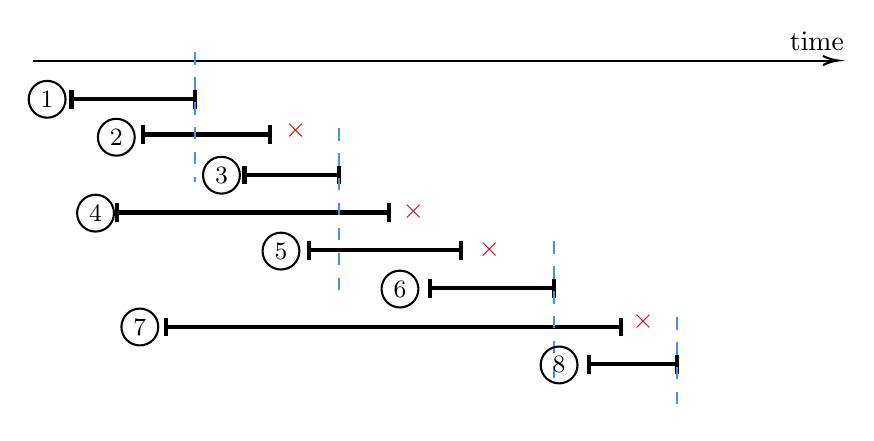
\begin{tikzpicture}[x=0.5pt,y=0.5pt,yscale=-1,xscale=1]
%uncomment if require: \path (0,309); %set diagram left start at 0, and has height of 309

%Straight Lines [id:da9015649955021968] 
\draw    (11,36) -- (591,36) ;
\draw [shift={(593,36)}, rotate = 180] [color={rgb, 255:red, 0; green, 0; blue, 0 }  ][line width=0.75]    (10.93,-3.29) .. controls (6.95,-1.4) and (3.31,-0.3) .. (0,0) .. controls (3.31,0.3) and (6.95,1.4) .. (10.93,3.29)   ;
%Straight Lines [id:da32866075720806565] 
\draw [line width=1.5]    (39,64) -- (128.5,64) ;
\draw [shift={(128.5,64)}, rotate = 180] [color={rgb, 255:red, 0; green, 0; blue, 0 }  ][line width=1.5]    (0,6.71) -- (0,-6.71)   ;
\draw [shift={(39,64)}, rotate = 180] [color={rgb, 255:red, 0; green, 0; blue, 0 }  ][line width=1.5]    (0,6.71) -- (0,-6.71)   ;

%Straight Lines [id:da254468097345411] 
\draw [line width=1.5]    (90.5,89.43) -- (182.5,89.43) ;
\draw [shift={(182.5,89.43)}, rotate = 180] [color={rgb, 255:red, 0; green, 0; blue, 0 }  ][line width=1.5]    (0,6.71) -- (0,-6.71)   ;
\draw [shift={(90.5,89.43)}, rotate = 180] [color={rgb, 255:red, 0; green, 0; blue, 0 }  ][line width=1.5]    (0,6.71) -- (0,-6.71)   ;

%Straight Lines [id:da3468808931598407] 
\draw [line width=1.5]    (164,118.86) -- (232.5,118.86) ;
\draw [shift={(232.5,118.86)}, rotate = 180] [color={rgb, 255:red, 0; green, 0; blue, 0 }  ][line width=1.5]    (0,6.71) -- (0,-6.71)   ;
\draw [shift={(164,118.86)}, rotate = 180] [color={rgb, 255:red, 0; green, 0; blue, 0 }  ][line width=1.5]    (0,6.71) -- (0,-6.71)   ;

%Straight Lines [id:da18209051305473312] 
\draw [line width=1.5]    (72,145.79) -- (268.5,145.79) ;
\draw [shift={(268.5,145.79)}, rotate = 180] [color={rgb, 255:red, 0; green, 0; blue, 0 }  ][line width=1.5]    (0,6.71) -- (0,-6.71)   ;
\draw [shift={(72,145.79)}, rotate = 180] [color={rgb, 255:red, 0; green, 0; blue, 0 }  ][line width=1.5]    (0,6.71) -- (0,-6.71)   ;

%Straight Lines [id:da8863435056826324] 
\draw [line width=1.5]    (210.5,173.22) -- (320.5,173.22) ;
\draw [shift={(320.5,173.22)}, rotate = 180] [color={rgb, 255:red, 0; green, 0; blue, 0 }  ][line width=1.5]    (0,6.71) -- (0,-6.71)   ;
\draw [shift={(210.5,173.22)}, rotate = 180] [color={rgb, 255:red, 0; green, 0; blue, 0 }  ][line width=1.5]    (0,6.71) -- (0,-6.71)   ;

%Straight Lines [id:da8287805623261496] 
\draw [line width=1.5]    (298,200.65) -- (387.5,200.65) ;
\draw [shift={(387.5,200.65)}, rotate = 180] [color={rgb, 255:red, 0; green, 0; blue, 0 }  ][line width=1.5]    (0,6.71) -- (0,-6.71)   ;
\draw [shift={(298,200.65)}, rotate = 180] [color={rgb, 255:red, 0; green, 0; blue, 0 }  ][line width=1.5]    (0,6.71) -- (0,-6.71)   ;

%Straight Lines [id:da032564250121786986] 
\draw [line width=1.5]    (107.5,228.58) -- (436,228.58) ;
\draw [shift={(436,228.58)}, rotate = 180] [color={rgb, 255:red, 0; green, 0; blue, 0 }  ][line width=1.5]    (0,6.71) -- (0,-6.71)   ;
\draw [shift={(107.5,228.58)}, rotate = 180] [color={rgb, 255:red, 0; green, 0; blue, 0 }  ][line width=1.5]    (0,6.71) -- (0,-6.71)   ;

%Straight Lines [id:da39810447379181857] 
\draw [line width=1.5]    (413,255.5) -- (476.5,255.5) ;
\draw [shift={(476.5,255.5)}, rotate = 180] [color={rgb, 255:red, 0; green, 0; blue, 0 }  ][line width=1.5]    (0,6.71) -- (0,-6.71)   ;
\draw [shift={(413,255.5)}, rotate = 180] [color={rgb, 255:red, 0; green, 0; blue, 0 }  ][line width=1.5]    (0,6.71) -- (0,-6.71)   ;

%Straight Lines [id:da46422592981377986] 
\draw [color={rgb, 255:red, 74; green, 144; blue, 226 }  ,draw opacity=1 ] [dash pattern={on 4.5pt off 4.5pt}]  (128.5,30) -- (128.5,124) ;
%Straight Lines [id:da6351884156456712] 
\draw [color={rgb, 255:red, 74; green, 144; blue, 226 }  ,draw opacity=1 ] [dash pattern={on 4.5pt off 4.5pt}]  (232.5,84.86) -- (232.5,202) ;
%Straight Lines [id:da33627378877589575] 
\draw [color={rgb, 255:red, 74; green, 144; blue, 226 }  ,draw opacity=1 ] [dash pattern={on 4.5pt off 4.5pt}]  (387.5,166.65) -- (387.5,273) ;
%Straight Lines [id:da20534568749266735] 
\draw [color={rgb, 255:red, 74; green, 144; blue, 226 }  ,draw opacity=1 ] [dash pattern={on 4.5pt off 4.5pt}]  (476.5,221.5) -- (476.5,289.5) ;

% Text Node
\draw (556,13) node [anchor=north west][inner sep=0.75pt]   [align=left] {time};
% Text Node
\draw    (88.38, 228.58) circle [x radius= 13.31, y radius= 13.31]   ;
\draw (88.38,228.58) node  [font=\small] [align=left] {$\displaystyle 7$};
% Text Node
\draw    (190.38, 173.72) circle [x radius= 13.31, y radius= 13.31]   ;
\draw (190.38,173.72) node  [font=\small] [align=left] {$\displaystyle 5$};
% Text Node
\draw    (56.38, 146.29) circle [x radius= 13.31, y radius= 13.31]   ;
\draw (56.38,146.29) node  [font=\small] [align=left] {$\displaystyle 4$};
% Text Node
\draw    (147.38, 118.86) circle [x radius= 13.31, y radius= 13.31]   ;
\draw (147.38,118.86) node  [font=\small] [align=left] {$\displaystyle 3$};
% Text Node
\draw    (21.38, 64) circle [x radius= 13.31, y radius= 13.31]   ;
\draw (21.38,64) node  [font=\small] [align=left] {$\displaystyle 1$};
% Text Node
\draw    (71.38, 91.43) circle [x radius= 13.31, y radius= 13.31]   ;
\draw (71.38,91.43) node  [font=\small] [align=left] {$\displaystyle 2$};
% Text Node
\draw    (276.38, 201.15) circle [x radius= 13.31, y radius= 13.31]   ;
\draw (276.38,201.15) node  [font=\small] [align=left] {$\displaystyle 6$};
% Text Node
\draw    (391.38, 256) circle [x radius= 13.31, y radius= 13.31]   ;
\draw (391.38,256) node  [font=\small] [align=left] {$\displaystyle 8$};
% Text Node
\draw (138,55) node [anchor=north west][inner sep=0.75pt]   [align=left] {$\displaystyle \textcolor[rgb]{0.29,0.56,0.89}{\checkmark }$};
% Text Node
\draw (191,78) node [anchor=north west][inner sep=0.75pt]   [align=left] {$\displaystyle \textcolor[rgb]{0.82,0.01,0.11}{\times }$};
% Text Node
\draw (276,136) node [anchor=north west][inner sep=0.75pt]   [align=left] {$\displaystyle \textcolor[rgb]{0.82,0.01,0.11}{\times }$};
% Text Node
\draw (331,164) node [anchor=north west][inner sep=0.75pt]   [align=left] {$\displaystyle \textcolor[rgb]{0.82,0.01,0.11}{\times }$};
% Text Node
\draw (442,216) node [anchor=north west][inner sep=0.75pt]   [align=left] {$\displaystyle \textcolor[rgb]{0.82,0.01,0.11}{\times }$};
% Text Node
\draw (244,111) node [anchor=north west][inner sep=0.75pt]   [align=left] {$\displaystyle \textcolor[rgb]{0.29,0.56,0.89}{\checkmark }$};
% Text Node
\draw (400,192) node [anchor=north west][inner sep=0.75pt]   [align=left] {$\displaystyle \textcolor[rgb]{0.29,0.56,0.89}{\checkmark }$};
% Text Node
\draw (486,244) node [anchor=north west][inner sep=0.75pt]   [align=left] {$\displaystyle \textcolor[rgb]{0.29,0.56,0.89}{\checkmark }$};


\end{tikzpicture}

